\section{Introduction}
\subsection{Definition}
{\bf Open-Source Intelligence (OSINT)} is a process for finding publicly available
information on a target company and/or individuals that allows identification
of events (i.e., public and private meetings), external and internal
dependencies, and connections. OSINT uses public (Open-Source) information from
freely available sources to obtain the desired results. 


The focus of OSINT lies in the word {\bf Intelligence}, which means
constructing relationships between individual pieces of information from which
we can create specific patterns and profiles about the target. The art here is
to look behind the scenes and think outside the box.

Open-source information or open sources, is any data that can be obtained from
public sources by anyone without any restrictions, whether for free or
commercially, in a legal and ethically acceptable way.

OSINT is based only on the passive gathering of information about the target
company from publicly available and (without registration or authentication
required) accessible sources. 


\subsection{Methodology}
To perform OSINT efficiently, we need a structure that shows us the essential
aspects and dependencies of the information resources and core information. The
following diagram shows the critical core elements required and can, of course,
contain additional components.

\begin{figure}
  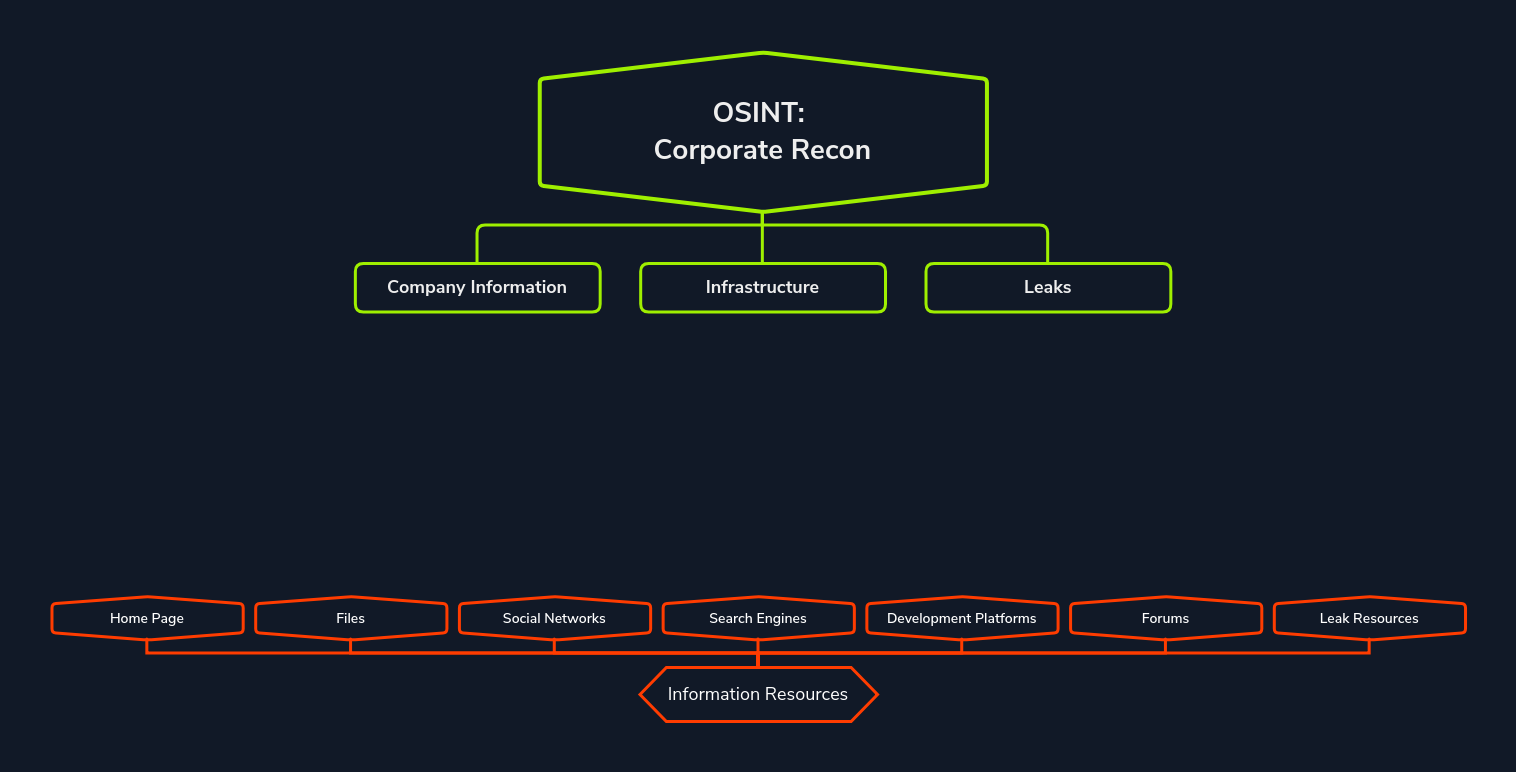
\includegraphics[width=\linewidth]{recon/osint/images/osint-structure.png}
  \caption{OSINT structure}
  \label{fig:osint-structure}
\end{figure}

Here we distinguish between the {\bf Core Elements} we need and the {\bf Information
Resources} from which we can extract the corresponding core information.

{\bf Core Elements} are pieces of information that give us a better picture of
the company and its infrastructure. These can be names and versions of software
applications, servers, names, user names, hashes, URLs, passwords, and much
more.

{\bf Information Resources} are resources from which we obtain these Core
Elements. These information resources can be websites, social networks,
documents, scripts, and many others.


we have to keep in mind that any information we find will lead to repeated
searches and new resources for more detailed information. 

Therefore, it is highly recommended to organize the whole process in {\bf
cycles} and repeat the search with the new information for each new cycle. This
systematic approach allows us to have a structured workflow and clean
documentation that will enable the client and us to understand precisely how
the data and information have been obtained.

When we use OSINT, we can divide our core information results into three categories:
\begin{verbatim}
Company Information 	Infrastructure 	                Leaks
Organization 	i       Domain Information 	            Archives
Locations 	            Public Domain Records 	        Internal Leaks
Staff 	                Domain Structure 	            Breaches
Contact Information 	Cloud Storage
Business Records 	    Email Addresses
Services 	            Third-Parties
Social Networks 	    Compounded Social Networks
                    	Technologies in Use
\end{verbatim}

In this methodology, we take a point from the information categories ({\bf Core
Elements}) and search for the relevant information for it through the different
{\bf information resources}.

Theoretically, the reverse procedure can be used too. However, it has a
significant disadvantage because we have many information resources to adapt
our methodology to, rather than our information resources to our methodology. 

The result is that we are left with an unstructured approach and are guided by
the information resources but not by the information results.

\subsubsection{Workflow}

{\emph It is essential to understand that, using this methodology, we adapt our
information resources to the methodology, not the methodology to our
information resources.}

In this way, we work according to an organized structure and get far more
results. It requires a little more effort to go through the same page several
times to cover different information areas and categories (Core Elements).
However, we maintain a structured and transparent methodology without
overlooking specific details relevant to a particular information area and
category. This also allows us to create clear and detailed documentation and
work in cycles independent of the cases.

To make this structured methodology efficient, we need to work with two browser
windows: 
\begin{itemize}
    \item {\bf Research Browser} use only for our research. Here we send all search
        requests and log the entire OSINT process. The research browser's
        history must be cleaned before use to prevent us from logging results
        from other companies. We can use the add-on called
        \href{https://github.com/jiacai2050/history-master}{History Master} to
        log our searches and finally export them as documentation.
    \item {\bf Resource Browser} serves as a summary of the information
        resources we find during the investigation. In this one, we move all
        the information resources to which we can return to search for
        information for other categories. For example, we will get to know
        development platforms containing leaks and names of employees or
        developers, email addresses, and usernames. In this part, we can also
        use the add-on called
        \href{https://addons.mozilla.org/en-US/firefox/addon/single-file/?utm_source=addons.mozilla.org&utm_medium=referral&utm_content=search}{SingleFile}.
        This allows us to copy the web pages with the information and save them
        locally as proof.
\end{itemize}

he actual process is quite simple, as we now split our results between two
browsers. So as soon as we have found a new information resource and examined
it in the Research Browser and discover that there is more useful information
there, we drag the newly opened tab to the Resource Browser, which we will turn
to later.


{\bf We document all our discoveries and structure them accordingly to each
phase and our cycle.}


\subsubsection{Logging}

To work efficiently and in a structured way, we must also document the results
and information we find clearly. However, we also need to log our steps and
prove how we found the information. With the two different browsers, we have
found a way to separate our search from the resources. To create clear
documentation, we need three components:
\begin{itemize}
        \item Visited websites
        \item Timestamp
        \item Queries
\end{itemize}

All of this information is stored in our browser history, and we can use it
quite efficiently for our purposes. A handy add-on for this is History Master.


Usefull tips :
\begin{itemize}
    \item export history-master to csv then \verb+csvtojson < history.csv | jq .+
    \item We can store all the websites locally using the SingleFile. This
        add-on offers an excellent way to download all open tabs with one
        click. Another great advantage of this is that these stored pages can
        also be searched locally \verb+cat *.html | html2text | grep "Emma Williams"+
\end{itemize}

\subsection{Business Investigation}
We should note down or at least keep in mind some questions that will help us
get a clear and efficient overview during our research. These questions will
also help us establish links between the individual pieces of information that
the actual intelligence piece of the phrase OSINT stands for.

\subsubsection{Company Information}
includes the company's general overview. This means
we will try to understand the company's structure:
\begin{itemize}
    \item  How many employees does the company have?
    \item  What is its objective?
    \item  How is the company positioned in society and the market?
    \item  How profitable is the company?
    \item  How does the company function?
    \item  How do they manage their tasks?
    \item  What services does the company provide?
    \item  How is the company positioned financially?
    \item  Which target group does the company pursue?
    \item  Where is the company located?
    \item  What are the physical security measures?
    \item  How do interaction and advertising with (potential) customers take place?
    \item  How strong is the company's reputation?
\end{itemize}

The process of staff investigation, can provide us with valuable information
that allows us to assess their knowledge and experience. It is a very
time-consuming stage to search for these people, as we first have to find all
the people then try to find everything relevant about them if allowed

In this search, we try to determine:
\begin{itemize}
    \item  What position do the employees hold?
    \item  Which departments exist within the company?
    \item  Their day-to-day tasks.
    \item  What are they responsible for?
    \item  What dependencies do the employee have?
\end{itemize}

Here we will only deal roughly with the individual employees. We will deal with
them more directly in another Module called {\bf OSINT: Staff Investigationr}.
It requires a slightly different approach to work with the information in an
efficient and structured way. Once we have gathered this information, we will
move on to profiling, which we will deal with more extensively in the {\bf OSINT:
Staff Profiling Module}.

Social networks are used for personal profiles and the sharing of information
from one's own private life. They are also used to publish products and news
that provide new information about the company and its technologies. Therefore,
in this phase, we try to determine:
\begin{itemize}
    \item Which products are being developed?
    \item Which technologies are utilized?
    \item Who are the developers?
    \item Which conferences do the employees attend?
    \item Where are these products used?
    \item Who uses these products and services?
\end{itemize}

For example, when new software is released and sold to thousands of companies,
it is interesting to get a demo of that software and analyze it for
vulnerabilities. If we can identify a vulnerability, all companies that use
this specific software version will also be affected by the vulnerability.

\subsubsection{Infrastructure}
we move into more technical details. Here we try to find
out:
\begin{itemize}
    \item  How is the company set up in terms of information technology?
    \item  Who are the administrators?
    \item  Does it meet the best possible security standards?
    \item  Which technologies are used?
    \item  What entries are there about the domain?
    \item  Which certificates can be obtained?
    \item  How many domains are registered to the company?
    \item  What is the ASN?
    \item  Which netblocks has the company reserved?
    \item  Which third-party providers are used, and for what?
    \item  How many and which servers are publicly accessible?
    \item  How many and which email addresses are available?
\end{itemize}

This gives us a much better understanding of the technologies and the technical
environment we have to deal with. Understanding how the entire company is
positioned from an infrastructure standpoint is essential for identifying
potential attack vectors. For example, specific configurations in the DNS
servers can give us a rough idea of how experienced our target company's
respective administrator is.


\subsubsection{Leaks}

Most of the data put on the internet is stored there for decades and can be
found easily. We can find different versions of the web servers and the
website's design, for example, or documents removed years ago that contained
up-to-date information about employees, technologies, or processes.

Internal leaks can be found on various forums. When a developer on
StackOverflow asks a question to solve a problem in their code, the code is
often shared with the others to give better insight into their issue. If the
developer is under a lot of pressure or distracted, they may accidentally post
code containing passwords or other sensitive data. The functions that the
developers are working on can be much more interesting. These may contain
vulnerabilities if inexperienced developers are employed to write specific
sections of code.
